
Zur Bestimmung der Schirmdämpfung elektromagnetischer Schirme gibt es je nach Anwendungsfall die unterschiedlichsten Normen und Verfahren, von denen im Folgenden eine Auswahl vorgestellt werden soll.
\par
\vspace{\linespace}
Anzumerken ist, dass die Reproduzierbarkeit von Messungen aufgrund von unterschiedlichen Geometrien der Testkammern, unterschiedlichen Antennencharakteristika und Abweichungen in der Prüfkörperkontaktierung trotz ähnlichem Aufbau unter Umständen sehr gering sein kann und Messunterschiede im Bereich von \SI{20}{\Dezibel} möglich sind. Je nach Güte des Aufbaus kann jedoch eine Wiederholbarkeit von Messungen mit Abweichungen kleiner als \SI{1}{\Dezibel} erreicht werden~\cite{EM_Schirmung}.
\par
\vspace{\linespace}
Gemeinsam haben alle vorgestellten Messmethoden, dass die Schirmdämpfung, wie im \Abschnitt\ref{cha:2_sub_Begriff_der_Schirmdaempfung} erwähnt, durch Vergleichsmessungen der Sende- und Ausgangspegel jeweils mit und ohne Schirm durchgeführt werden. 


\subsection{Messzellen zur Messung der Intrinsic-Schirmdämpfung}

Die als Intrinsic-Schirmdämpfung bezeichnete Materialeigenschaft, elektromagnetische Feld zu dämpfen, wird aufgrund des einfachen Aufbaus und der guten Vergleichbarkeit von Messungen in einer TEM-Messzelle nach dem ASTM-Standard D4935 bestimmt~\cite{ASTM_D4935, Measurement_Shielding_Textile_Materials_Free_Space_Transmission}. Vereinfacht besteht die Messzelle aus einer aufgeweiteten Koaxialleitung, in welche eine Materialprobe senkrecht der Ausbreitungsrichtung eingefügt wird~\cite{EM_Schirmung, Handbook_EMI_Vol_3}. Da hierbei $\vec E$- und $\vec H$-Feldvektor parallel zur Probe ausgerichtet sind, wird auch von einer Fernfeld-Simulation gesprochen~\cite{Techniques_Shielding_Effectiveness_Far_Field_Simulation, EMV}. Problematisch bei dieser Messmethode ist vor allem die korrekte Kontaktierung der Probe~\cite{EM_Schirmung} und dass keine Breitbandmessungen durchgeführt werden können, d.h. für jeden Frequenzbereich eine eigene Messzelle mit bestimmten Maßen erforderlich ist~\cite{Techniques_Shielding_Effectiveness_Far_Field_Simulation, EMV}. Weiterhin können hierbei keine unterschiedlichen Polarisationen getestet werden~\cite{Techniques_Shielding_Effectiveness_Far_Field_Simulation}. Für Messungen über \SI{1,6}{\giga\hertz} ist die TEM-Messzelle darüber hinaus kaum geeignet, da es zur Ausbildung höherer Moden kommt~\cite{EMV}. In~\cite{Measurement_Electromagnetic_Shielding_Effectiveness_Composite_Carbon_Nickel_Thinfilm} wurde diese Methode beispielsweise nur für Messungen bis \SI{1,5}{\giga\hertz} genutzt.
%Grenzfrequenz bei 1,6 GHz (cite(EMV)) durch Ausbildung höherer Moden
\par
\vspace{\linespace}
Weitere Methoden zur Bestimmung der Intrinsic-Schirmdämpfung sind die Dual-Chamber Box in Anlehung an den ASTM-Standard ES7-83~\cite{ASTM_ES7-83} und die Doppel-TEM-Messzelle. Da beide jedoch vor allem bei Frequenzen im Gigahertz-Bereich eine stark inhomogene Feldverteilung aufweisen, werden diese hier nicht in Betracht gezogen~\cite{EM_Schirmung, EMV}.


\subsection{Genormte Messverfahren für Gehäuse und Räume}\label{cha:2_sub_Genormte_Messverfahren}

\subsubsection{DIN EN 61000-5-7}

Die DIN 61000-5-7 \cite{DIN_EN_61000-5-7} beschreibt die Messung von Schirmdämpfungen im Bereich von \SI{10}{\kilo\hertz} bis \SI{40}{\giga\hertz} in Anlehnung an die Störfestigkeitsprüfung nach DIN 61000-4-3 \cite{DIN_EN_61000-4-3}.
\par
\vspace{\linespace}
Die Messung wird dabei in einer geschirmten Kabine durchgeführt oder alternativ auf einem offenen Testgelände, d.h. einem Freifeld, mit mindesten \SI{5}{\meter} Abstand zu jeglichem leitfähigem Material. Die Schirmkabine ist oberhalb von \SI{10}{\mega\hertz} mit Absorbern auszustatten. Die Feldhomogenität hat unabhängig vom Messplatz an der Vorderkante des Prüflings dabei \SI{3}{\Dezibel} zu betragen. Weiterhin sind die in \Abb\ref{fig:2_Schematik_Schirmdaempfungsmessung_DIN_61000-5-7} gekennzeichneten Maße für unterschiedliche Messfrequenzen und die zu verwendenden Antennenbauformen festgelegt. Oberhalb von \SI{1}{\giga\hertz} sind nach~\cite{DIN_EN_61000-5-7} Hornstrahler mit Kabeln zu verwenden, deren Kopplungsdämpfung \SI{10}{\Dezibel} oberhalb der gemessenen Schirmdämpfung liegt.


\begin{figure}[ht]
    \centering
    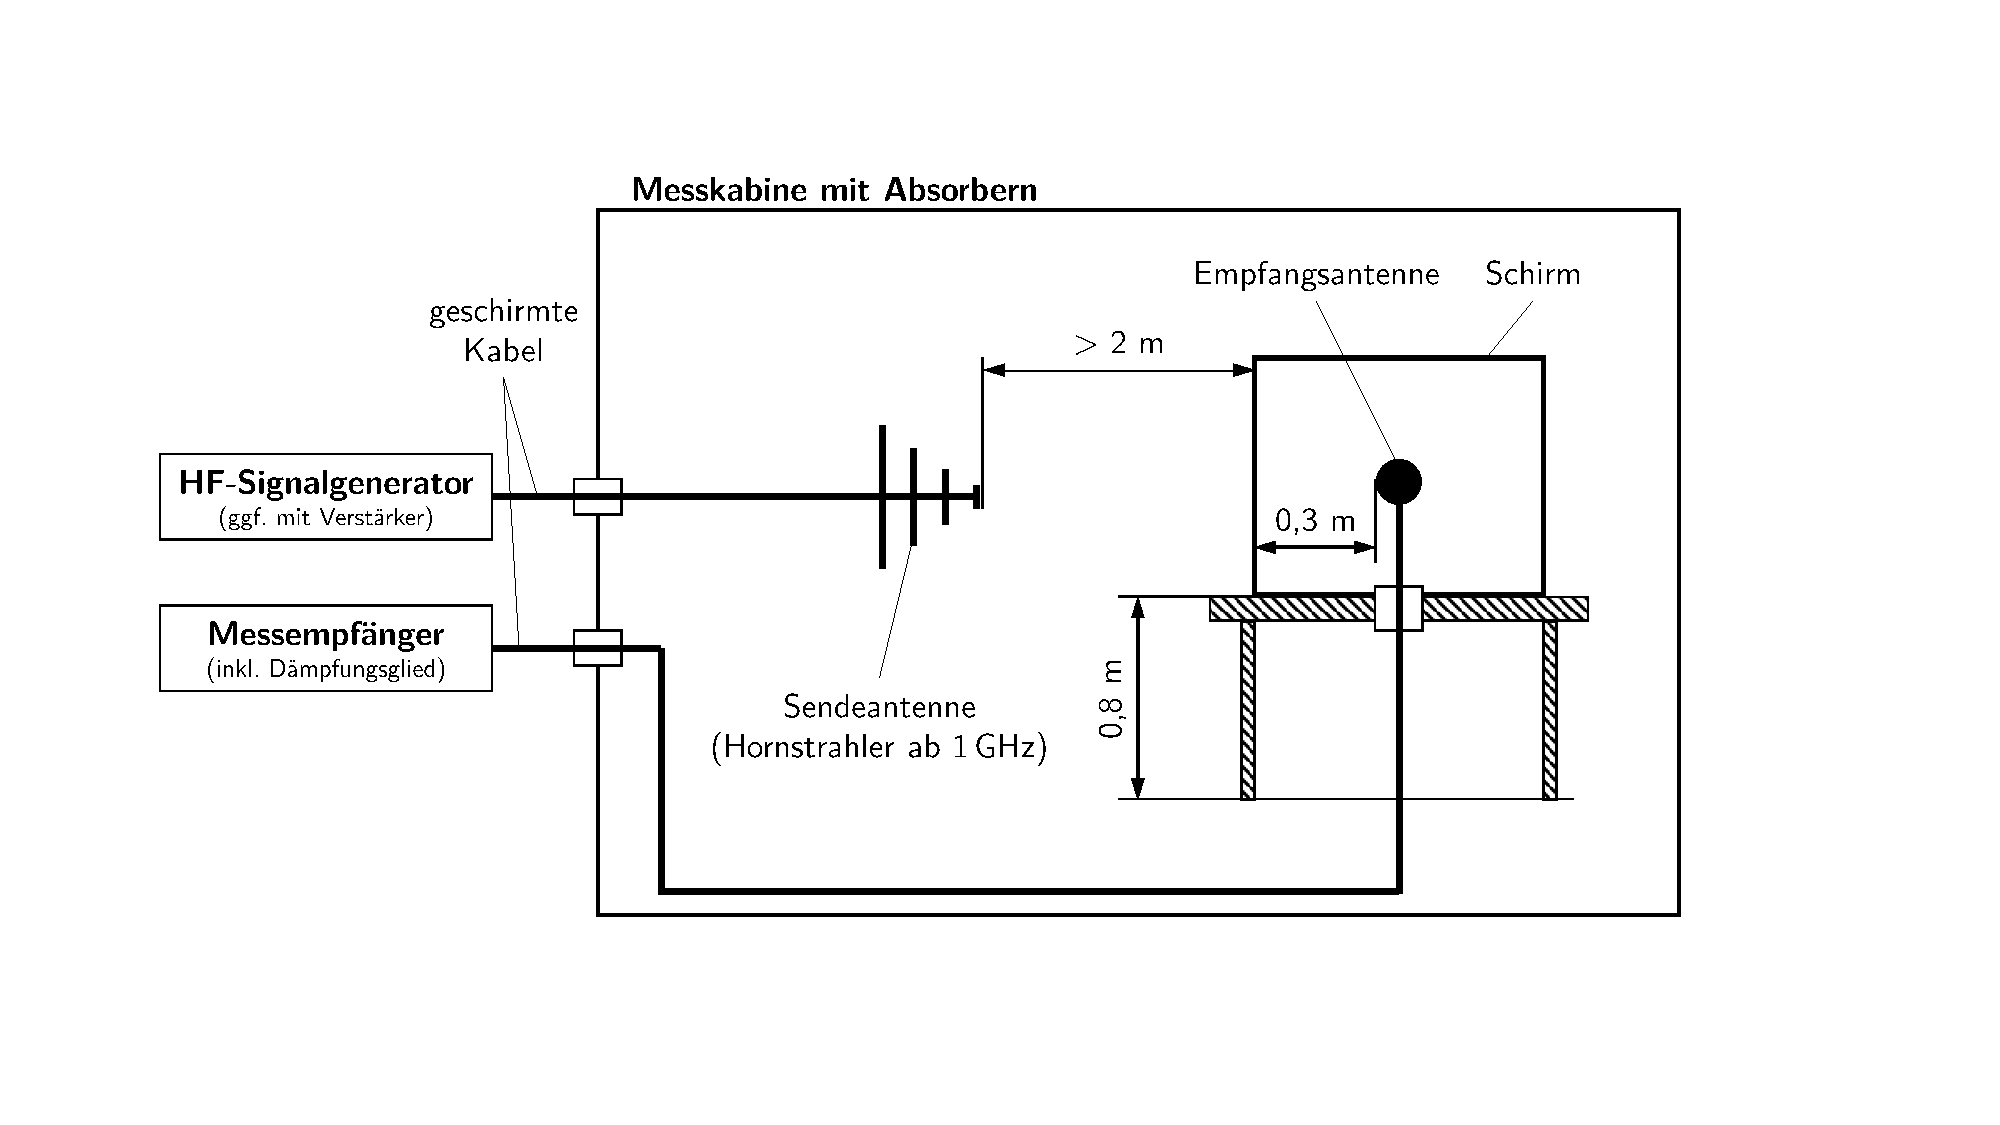
\includegraphics[page = 1, trim = 2cm 3cm 5cm 3cm, clip, width=.9\textwidth]{Abbildungen/Kapitel2/Schematiken_Schirmdaempfungsmessung.pdf}
    \caption[Schematischer Messaufbau der Schirmdämpfungsmessung nach \citeauthor{DIN_EN_61000-5-7} im Frequenzbereich zwischen \SI{1}{\giga\hertz} bis \SI{40}{\giga\hertz}]{Schematischer Messaufbau der Schirmdämpfungsmessung nach \citeauthor{DIN_EN_61000-5-7} im Frequenzbereich zwischen \SI{1}{\giga\hertz} bis \SI{40}{\giga\hertz} nach~\cite{DIN_EN_61000-5-7}}
    \label{fig:2_Schematik_Schirmdaempfungsmessung_DIN_61000-5-7}
\end{figure}


%Anpassung bei hohen Frequenz hinsichtlich Maße

\subsubsection{IEEE 299}
Im Vergleich zur DIN 61000-5-7 soll ebenfalls kurz auf die IEEE 299~\cite{IEEE_299} eingegangen werden, welche die Messung der Schirmdämpfung von Messkabinen und Räumen bis zu einem Frequenzbereich bis \SI{18}{\giga\hertz} beschreibt und den häufig zitierten Standard MIL-STD~285 abgelöst hat~\cite{EM_Schirmung}. Der in \Abb\ref{fig:2_Schematik-Schirmdaempfungsmessung_IEEE_299} gezeigte Messaufbau wird hier sowohl für den Frequenzbereich \SI{20}{\mega\hertz} bis \SI{300}{\mega\hertz}, also auch für den Hochfrequenzbereich ab \SI{300}{\mega\hertz} verwendet, wobei davon ausgegangen wird, dass sich die Schirmung ab \SI{300}{\mega\hertz} im Fernfeld der Antennen befindet und damit nahezu nur ebene Wellen geschirmt werden~\cite{EM_Schirmung, IEEE_299}. In der abgelösten Norm MIL-STD~285 wird im Gegensatz zur echten Einfügungsmessung der IEEE~299 die Empfangsantenne bei sonst ähnlichem Aufbau jeweils vor und hinter dem Schirm platziert~\cite{EM_Schirmung}.
\par
\vspace{\linespace}
Die DIN~50147"~1~\cite{DIN_EN_50147-1} beschreibt ein ähnliches Messverfahren zur IEEE~299, jedoch vor allem im Kontext von Absorberhallen.  

\begin{figure}[ht]
    \centering
    \includegraphics[page = 2, trim = 2cm 3cm 4cm 3cm, clip, width=.9\textwidth]{Abbildungen/Kapitel2/Schematiken_Schirmdaempfungsmessung.pdf}
    \caption[Schematischer Messaufbau der Schirmdämpfungsmessung nach \citeauthor{IEEE_299} für Frequenzen ab \SI{20}{\mega\hertz}]{Schematischer Messaufbau der Schirmdämpfungsmessung nach \citeauthor{IEEE_299} für Frequenzen ab \SI{20}{\mega\hertz} nach~\cite{IEEE_299}}
    \label{fig:2_Schematik-Schirmdaempfungsmessung_IEEE_299}
\end{figure}


\subsection{Modenverwirbelungskammer}
Eine Alternative zur Messung in einer mit Absorbern ausgestatteten Kabine stellt die Messung der Schirmdämpfung in einer Modenverwirbelungskammer~(\acsu{MSC}) dar~\cite{EMV}. Hier werden die Resonanzfrequenzen der Messkabine (vgl. \Abschnitt\ref{cha:2_subsub_Hohlraumresonanzen}) mithilfe beweglicher Metallplattenstrukturen so verändert, dass es im Betrieb nicht zu stehenden Wellen kommt und Hohlraumresonanzen somit nicht auftreten. Dafür müssen jedoch die Kammer und der sogenannte Modenrührer gut aufeinander abgestimmt sein und es muss eine entsprechend hohe Modendichte im gewünschten Messintervall vorliegen. 
\par
\vspace{\linespace}
Bei Schirmdämpfungsmessungen von Gehäusen haben \acp{MSC} den Vorteil der kurzen Messzeit, weil keine Drehung des Prüflings notwendig ist. Sie bieten untereinander eine gute Vergleichbarkeit, da kleine Unterschiede im Messaufbau nur von geringer Bedeutung sind. Messungen in reinen Absorberkammern lassen sich jedoch mit denen aus \acp{MSC} kaum vergleichen~\cite{EMV}. Weiterhin ist die Auswertung der Messwerte deutlich komplexer und die Feldverteilung ist aufgrund der vielen erzwungenen Reflexionen quasi nicht bestimmbar~\cite{EMV}. Die Messwerte haben hier nur im Kontext einer zeitlichen Mittelung eine Aussagekraft~\cite{EMV}.


%siehe EMV 
\subsection{Auswahl der geeigneten Messmethode}
Aufgrund der erwähnten nutzbaren oberen Grenzfrequenz von etwa \SI{1,6}{\giga\hertz} für die Messungen mit TEM-Messzellen sind diese und ähnliche Messaufbauten im Rahmen dieser Arbeit nicht sinnvoll nutzbar. Weiterhin überwiegen für den vorliegenden Anwendungsfall auch bei \acp{MSC} die erwähnten Nachteile, sodass diese als Konzept für die zu entwickelnde Messkammer ebenfalls verworfen wurden. 
\par
\vspace{\linespace}
Die Messung in einer Absorberkammer durch Einfügung der Prüflinge in die Signalstrecke zweier Antennen in Anlehnung an die DIN EN 61000-5-7 und IEEE 299~\cite{DIN_EN_61000-5-7, IEEE_299} stellt somit nach dem betrachteten Stand der Wissenschaft und für die vorliegenden Anforderungen an den Aufbau die beste Methode zur Ermittlung der Schirmdämpfung von Materialproben im Fernfeld dar. Im folgenden Kapitel~\ref{cha:3} wird der Entwurf im Detail dargelegt.







%Entscheidung für Absorberkammer mit Reflektor (ähnlich wie in Textil-Quelle) und Maßen in Anlehnung an Norm  



